\documentclass{article}
\author{Richard Gendal Brown, James Carlyle, Ian Grigg, Mike Hearn}
\date{August, 2016}
\title{Corda: An Introduction}
%%\setlength{\parskip}{\baselineskip}
\usepackage{amsfonts}
\usepackage{listings}
\usepackage{color}
\usepackage{epigraph}
\usepackage{graphicx}
\graphicspath{ {images/} }
\usepackage[export]{adjustbox}
\usepackage{float}
\usepackage{hyperref}
\usepackage[super,comma,sort&compress]{natbib}
\usepackage[nottoc]{tocbibind}
%\usepackage[natbibapa]{apacite} 
\renewcommand{\thefootnote}{\alph{footnote}}

%\epigraphfontsize{\small\itshape}
\setlength\epigraphwidth{4.5cm}
\setlength\epigraphrule{0pt}

\begin{document}

\maketitle 
%\epigraphfontsize{\small\itshape}

%\renewcommand{\abstractname}{An introduction}
%\textit{Confidential: Pre-Publication Final Draft For R3 Distributed Ledger Group Steering Committee}


\begin{abstract}

A distributed ledger made up of mutually distrusting nodes would allow for a single global database that records the state of deals and obligations between institutions and people. This would eliminate much of the manual, time consuming effort currently required to keep disparate ledgers synchronised with each other. It would also allow for greater levels of code sharing than presently used in the financial industry, reducing the cost of financial services for everyone. We present Corda, a platform which is designed to achieve these goals. This paper provides a high level introduction intended for the general reader. A forthcoming technical white paper elaborates on the design and fundamental architectural decisions.
\end{abstract}
\newpage
\tableofcontents
\newpage
\section{Introduction}
At R3, we believe that distributed ledger technology has the potential to transform the financial services industry to the benefit of its clients and participant firms alike. We envision a future where financial agreements are recorded and automatically managed without error, where anybody can transact seamlessly for any contractual purpose without friction. We believe markets will move towards models where parties to financial agreements record them once and collaborate to maintain accurate, shared records of these agreements. Duplications, reconciliations, failed matches and breaks will be things of the past. Isolated islands of asset representations will be no more.

We aspire to define a shared ledger fabric for financial services use-cases that can be deployed within existing legal frameworks and which relies on proven technologies. Our philosophy can be broken down into three categories: engineering for the requirements of institutions, a focus on non-functional requirements, and extensibility.

This paper introduces the design features of the Corda platform which we believe make it an attractive choice for regulated financial institutions.\footnote{The authors can be reached via email: Richard Gendal Brown \href{mailto:richard@r3cev.com}{(richard@r3cev.com)}, James Carlyle \href{mailto:james@r3cev.com}{(james@r3cev.com)}, Ian Grigg \href{mailto:iang@r3cev.com}{(iang@r3cev.com)}, Mike Hearn \href{mailto:mike@r3cev.com}{(mike@r3cev.com)}}

\section{Context}
Banks were amongst the earliest adopters of information technology and, contrary to popular belief, they have done a good job in automating previously manual processes and in digitizing previously physical processes. However, there are significant opportunities to improve the cost and efficiency of the architectures that emerged. 

In particular, each financial institution maintains its own ledgers, which record that firm's view of its agreements and positions with respect to its customer set and its counterparts. Its counterparts, in turn, maintain their views. This duplication can lead to inconsistencies, and it drives a need for costly matching, reconciliation and fixing of errors by and among the various parties to a transaction. To the extent that differences remain between two firms' views of the same transaction, this is also a source of risk, some of it potentially systemic.

A plurality of financial institutions drives competition and choice but the plurality of technology platforms upon which they rely drives complexity and creates operational risk. However, until recently, this was unavoidable: except for centralised market infrastructures\footnote{Examples of this include the Depository Trust \& Clearing Corporation (DTCC) and Continuous Linked Settlement Group (CLS).}, there were few effective ways to consolidate technology across firms without also consolidating the firms themselves.

Centralised market infrastructure utilities have gone some way towards increasing the amount of data and business-logic sharing between firms\footnote{Many market infrastructure utilities are actively studying the technical approaches discussed in this paper\cite{DTCC}.} but, overall, the degree of integration achieved in the realm of financial transactions still lags far behind that which has been achieved in the realm of information exchange since the advent of the web. \cite{IT}

We believe that the maturation of cryptographic techniques, exemplified in part by what is commonly referred to as ``blockchain technology", provides a new opportunity: the possibility of authoritative systems of record that are securely shared between firms. This vision provides the opportunity to transform the economics of financial firms, particularly but not exclusively in post-trade services, by implementing a new shared platform for the recording of financial events and processing of business logic: one where a single global logical ledger is authoritative for all agreements between firms recorded on it. This architecture will define a new shared platform for the industry, upon which incumbents, new entrants and third parties can compete to deliver innovative new products and services. 

\begin{figure}[H]
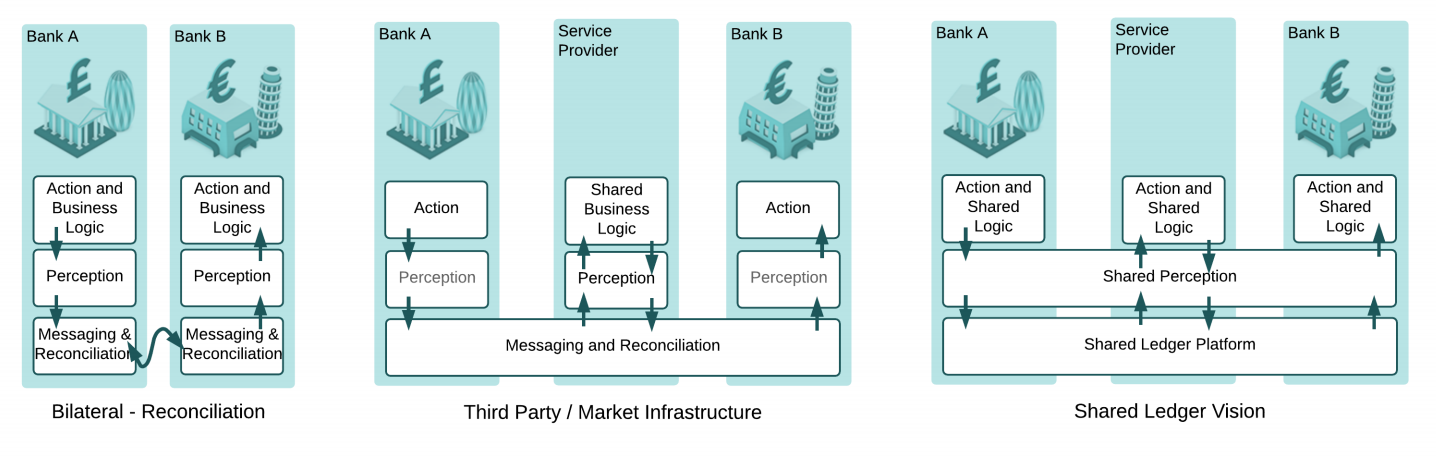
\includegraphics[scale=.5, center]{sharedlogic} 
\caption{In the diagram above, we show a progression from a world where parties to shared facts record and manage their own records, with associated discrepancies and duplications (\textit{``Bilateral - Reconciliation"}) or one where parties delegate control and responsibility over critical processing to centralised utilities (\textit{``Third Party / Market Infrastructure"}), to one where they collaborate to maintain a shared record, assured to be consistent between them, consuming the services of existing and new service providers and market infrastructure providers on an open and competitive basis (\textit{``Shared Ledger Vision"}).}
\end{figure}


We believe that the savings accruing from higher-quality data, fewer discrepancies and quicker agreement of details between firms will be significant. Moreover, deployment of this common architecture across firms will define a new platform on which existing and new providers can compete to serve the needs of clients. Going further, it is possible that such a platform will also find application within firms, where the problem of multiple systems recording details of the same trades is also a major driver of cost and complexity.

\section{Vision}
In the long-term, one can envision a ``global logical ledger" with which all economic actors will interact and which will allow any parties to record and manage agreements amongst themselves in a secure, consistent, reliable, private and authoritative manner. We say it is global in the sense that everybody sees the same data that pertains to them and logical in the sense that the physical implementation may be composed differently. As such, a possible end-state is one in which we have moved from authoritative systems-of-record maintained within firms to global authoritative systems-of-record shared \textit{between} firms. 

\subsection{End-State Principles}
Principles underpinning a possible end-state using distributed ledger technology may include:
\begin{itemize}
	\item Facts recorded by the ledger are, by contract, accepted as admissible evidence and legally binding by all parties in any dispute.
	\item Facts recorded by the ledger are regarded as authoritative rather than ``shadows" of authoritative data held elsewhere, enabling settlement to take place directly across the platform.
	\item Once all parties to an agreement have assented, facts recorded on the ledger are final and immutable\footnote{By ``immutable", we mean that attempts to tamper with previously committed records will be evident and will be rejected}; errors and unwinds must be processed through a subsequent transaction. Firms will be under pressure to re-engineer their internal processes to increase accuracy and quality.
	\item Any authorized actor may, in principle, connect directly to the ledger and use it to record agreements with its counterparts. No actor is compelled to deal with any other but we may see a decline in ``tiered" or hierarchical market models. 
	\item By promoting open standards and inclusive access, existing and new service providers can connect and compete to offer differentiated services, promoting choice and competition.
	\item The only parties who should have access to the details of a financial transaction are those parties themselves and others with a legitimate need to know.
\end{itemize}

However, the vision encompasses the notion of interim states, such as those that focus first on the sharing only of business logic. This is intended to acknowledge the reality that today's systems will be with us for the foreseeable future, requiring co-existence, integration and migration paths as a fundamental part of the solution design. These interim states can also deliver considerable value whilst legal and other non-technical implications of the longer-term vision are addressed in parallel.

It should be stressed that the long-term vision of a global logical ledger is intended to set a direction of travel but that its realization may be in the form of a multiplicity of ledgers. Perhaps this will take the form of one ledger per asset class which would be autonomous, loosely coupled, providing functional and operational independence between different business services. 

Architectural and strategic choices underpinning the vision include:
\begin{itemize} 
\item Records managed by this system will be accessible only to those actors with a legitimate interest in the assets and agreements they manage.
\item The behavior of agreements managed by the system will be described in computer code that explicitly refers to and gains its legitimacy from over-arching legal prose.\cite{Ricardian}
\item Support for contract code upgrades and explicit reference to dispute resolution procedures will be supported in order to provide certainty in the presence of failed contracts. This is because contractual disputes can occur, even in automated settings, as a result of both technical and human factors. 
\item Successful delivery of this vision will be through reduction of cost, risk and regulatory burden (including capital, liquidity and operational obligations) and through enabling of innovative new products and services.
\item To gain wide adoption across the financial community, portions of the system must and will be open: open source, open development process, open standards.
\item Although this vision talks in terms of a ``platform" or ``system", our belief is that the design will actually be multi-layered with different providers potentially competing/collaborating to deliver different pieces. Readers should not assume that we envisage a monolithic vertically integrated approach.
\item The vision also includes the possibility that higher-level layers of the “stack” can contain IP proprietary to individual firms or groups.
\item This system will operate under the assumption of an adversarial security environment: the growing threat of cybercrime must be taken as a given.
\end{itemize}

It is believed that the fundamental inventions needed to deliver this vision already exist. These include, but are not limited to, robust cryptography, global communications networks, standards for the definition of financial instruments and effective algorithms to ensure consistency at a global scale. 

What makes this vision possible today is that the recent popular interest in distributed ledger and blockchain systems has created an environment in which such a vision can be openly discussed and that a collaborative alliance through which multiple financial institutions can act together has been formed. It assumes an identity infrastructure between the participants in the network but makes no assumption as to its sophistication or mode of operation. Regulatory engagement is a key element of the design process.

From our requirements analysis and assessment of existing distributed ledger platforms, we concluded that no existing platform met our needs.  In essence, the threat models underpinning the designs of traditional distributed databases were unsuitable for our use-case of bringing mutually distrusting legal entities into consensus; and the architectures of existing blockchain systems were unsuitable for our requirement of restricted and carefully specified data sharing at the level of individual legal agreements.  As a result we designed and began development of Corda.

\section{Corda}
Corda is a distributed ledger platform for recording and processing financial agreements, designed to implement the vision contained in this document.  

The Corda platform supports smart contracts, matching the definition of Clack, Bakshi, Braine.\cite{SCT}  Our smart contract is an agreement whose execution is both \textit{automatable} by computer code working with human input and control, and whose rights and obligations, as expressed in legal prose, are legally \textit{enforceable}.  The smart contract links business logic and business data to associated legal prose in order to ensure that the financial agreements on the platform are rooted firmly in law and can be enforced and that we have a clear path to follow in the event of ambiguity, uncertainty or dispute.

\subsection{Principal Features}
Corda is specialized for use with regulated financial institutions. It is heavily inspired by blockchain systems, but without the design choices that make traditional blockchains inappropriate for many financial scenarios. 

Corda provides a framework to run smart contracts with these key activities and features:
\begin{itemize}
    \item{Recording and managing the evolution of financial agreements and other shared data between two or more identifiable parties in a way that is grounded in existing legal constructs and compatible with existing and emerging regulation}
    \item{Choreographing workflow between firms without a central controller.}
    \item{Supporting consensus between firms at the level of individual deals, not a global system.}
    \item{Supporting the inclusion of regulatory and supervisory observer nodes.}
    \item{Validating transactions solely between parties to the transaction.}
    \item{Supporting a variety of consensus mechanisms.}
    \item{Recording explicit links between human-language legal prose documents and smart contract code.}
    \item{Using industry-standard tools.}
    \item{Restricting access to the data within an agreement to only those explicitly entitled or logically privileged to it.}
\end{itemize}
These features contribute to the design of a platform appropriate for use in complex, financial services organizations. Note that this design does not use a native cryptocurrency or impose a global transaction speed limit.

\subsection{Concepts}
We begin with the idea of a global ledger: a reliable single source. However, in our model, it is not the case that transactions and ledger entries are globally visible. In cases where transactions only involve a small subgroup of parties we strive to keep the relevant data purely within that subgroup. 

The foundational object in our concept is a \textit{state object}, which is a digital document which records the existence, content and current state of an agreement between two or more parties. It is intended to be shared only with those who have a legitimate reason to see it. To ensure consistency in a global, shared system where not all data is visible to all participants, we rely heavily on secure cryptographic hashes to identify parties and data. The ledger is defined as a set of immutable state objects.

We talk and think in terms of the state of agreements and our objective is to ensure that all parties to the agreement remain in consensus as to this state as it evolves. One could argue that this is the essence of the blockchain concept: ensuring that the data held by different actors is, and remains, consistent as operations are applied to update that data, and that this forms the foundation on which reliable transactions are built: from simple monetary payments to sophisticated smart contract transitions.

\begin{figure}[H]
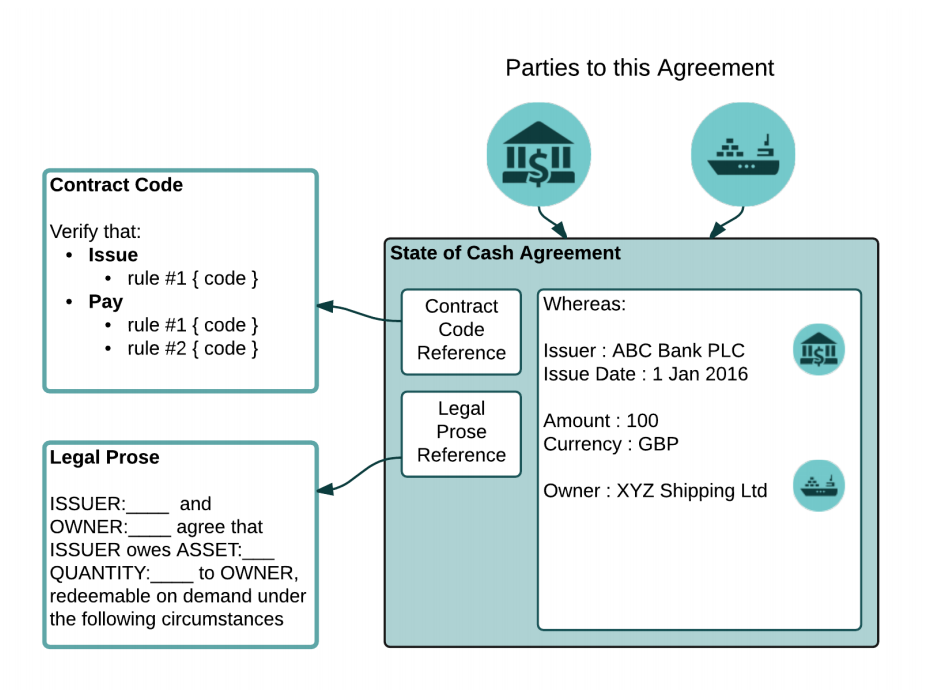
\includegraphics[scale = .4, center]{partiesto}
\caption{In the diagram above, we see a State object representing a cash claim of \pounds100 against a commercial bank, owned by a fictional shipping company.  The state object explicitly refers by hash to its governing legal prose and to the contract code that governs its transitions.}
\end{figure}

Our focus on states of agreements is in contrast to systems where the data over which participants much reach consensus is the state of an entire ledger or the state of an entire virtual machine. Corda provides three main tools to achieve global distributed consensus:
\begin{itemize}
    \item Smart contract logic to ensure state transitions are valid according to the pre-agreed rules.
    \item Uniqueness and timestamping services to order transactions temporally and eliminate conflicts.
    \item An orchestration framework which simplifies the process of writing complex multi-step protocols between multiple different parties.
    \end{itemize}
    
\subsection{Consensus}
In Corda, updates are applied using \textit{transactions}, which consume existing state objects and produce new state objects. There are two aspects of consensus:
\begin{enumerate}
\item{Transaction validity: parties can reach certainty that a proposed update transaction defining output states is valid by checking that the associated contract code runs successfully and has all the required signatures; and that any transactions to which this transaction refers are also valid.}
\item{Transaction uniqueness: parties can reach certainty that the transaction in question is the unique consumer of all its input states. That is: there exists no other transaction, over which we have previously reached consensus (validity and uniqueness), that consumes any of the same states.}
\end{enumerate}

Parties can agree on transaction validity by independently running the same contract code and validation logic. However, consensus over uniqueness requires a predetermined observer, which in many cases will be required to be independent.

\begin{figure}[H]
    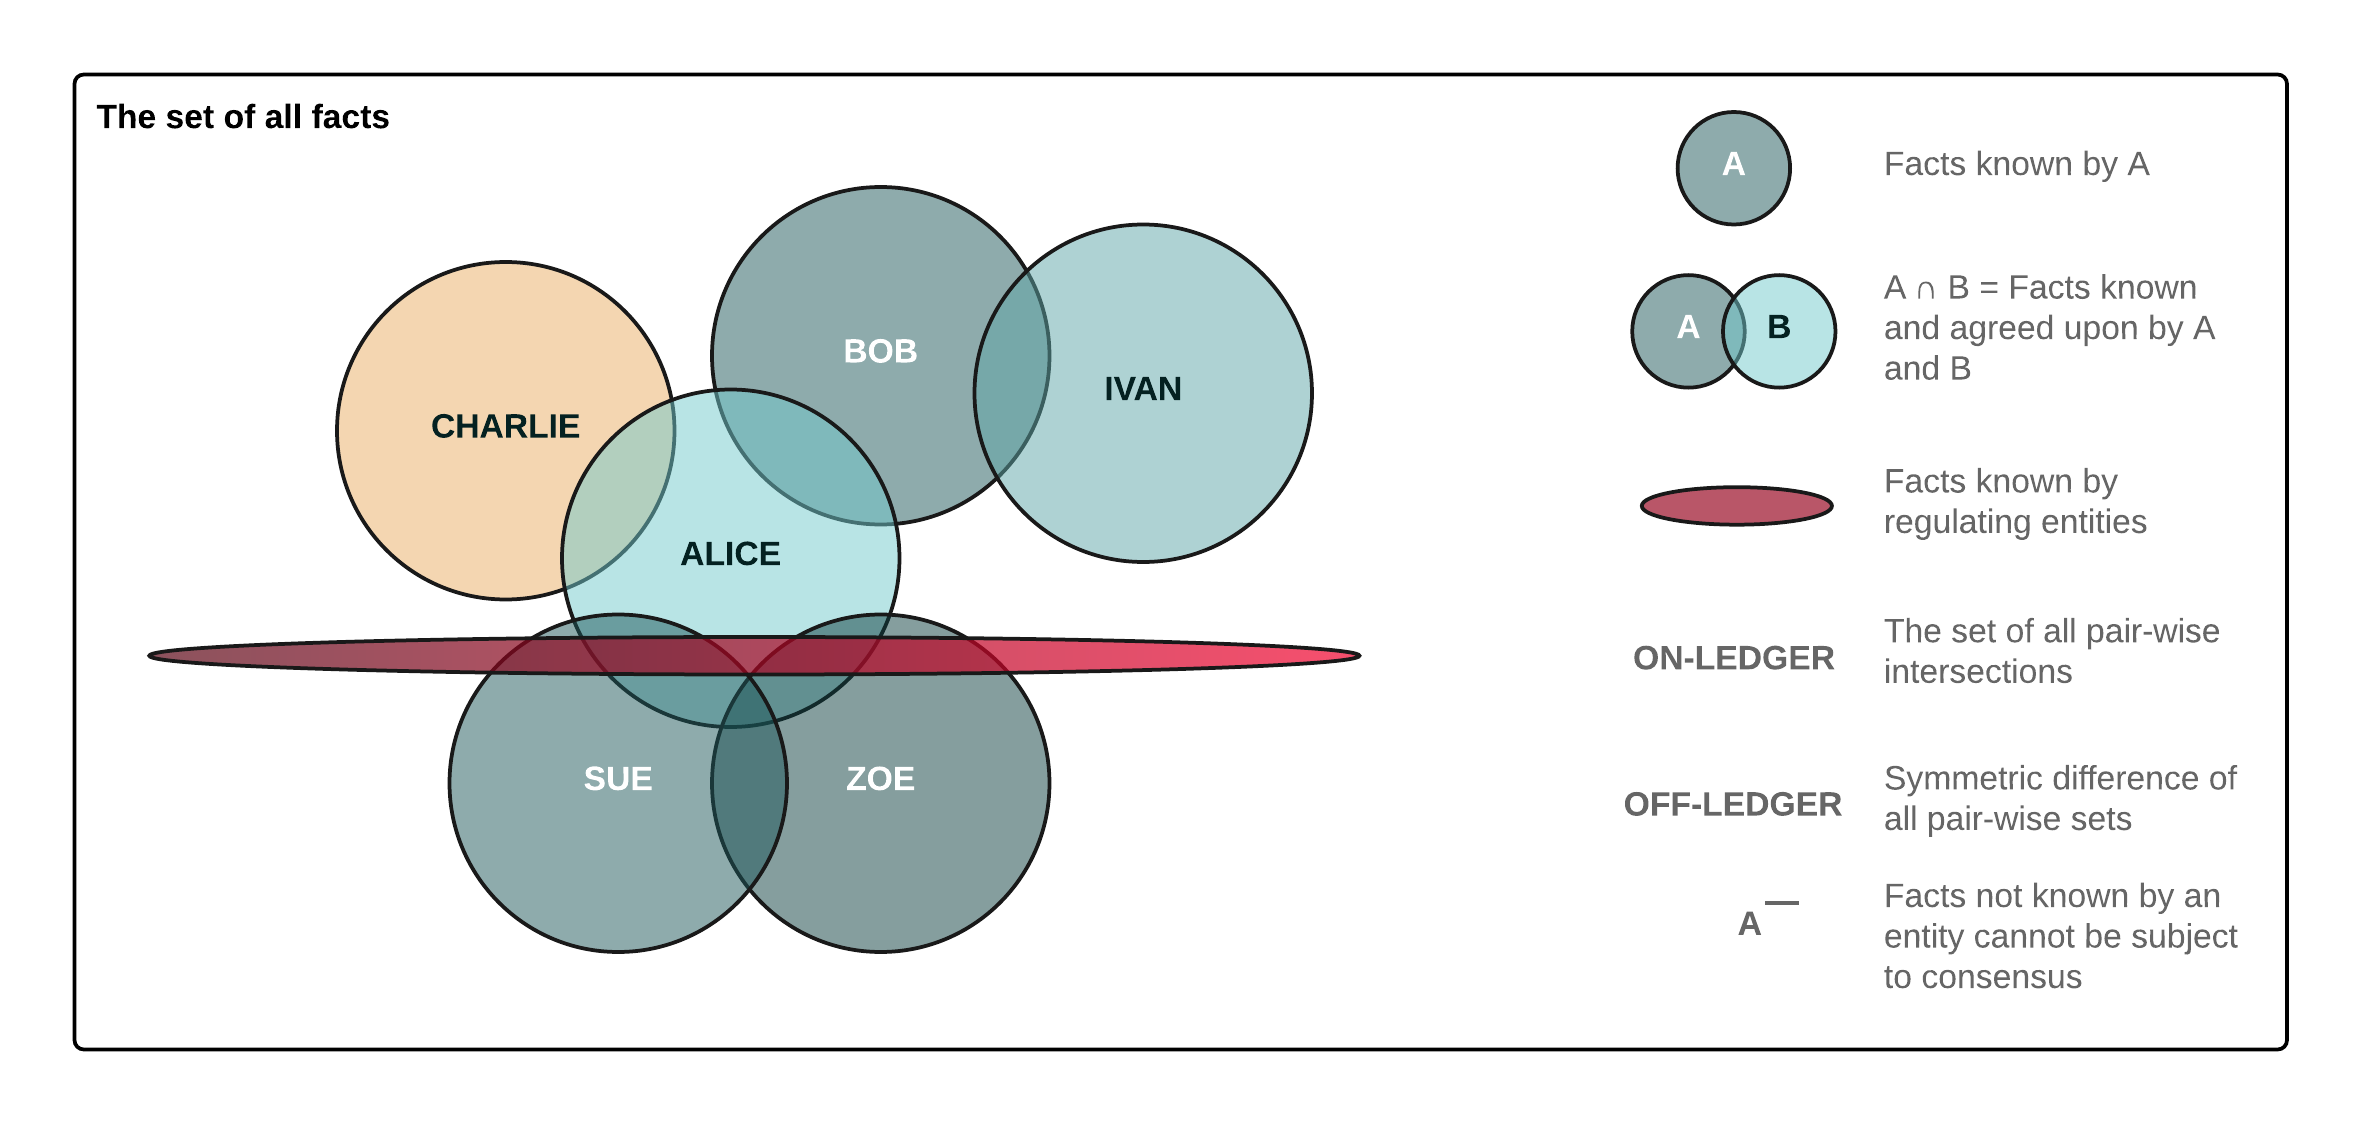
\includegraphics[scale = .5, center]{Consensus}
    \caption{Consensus over transaction validity is performed only by parties to the transaction in question. Therefore, data is only shared with those parties which are required to see it. Other platforms generally reach consensus at the ledger level. Thus, any given actor in a Corda system sees only a subset of the overall data managed by the system as a whole. We say a piece of data is ``on-ledger" if at least two actors on the system are in consensus as to its existence and details and we allow arbitrary combinations of actors to participate in the consensus process for any given piece of data. Data held by only one actor is ``off-ledger".}
\end{figure}

Corda has ``pluggable" uniqueness services. This is to improve privacy, scalability, legal-system compatibility\cite{EUC} and algorithmic agility. A single service may be composed of many mutually untrusting nodes coordinating via a byzantine fault tolerant algorithm, or could be very simple, like a single machine. In some cases, like when evolving a state requires the signatures of all relevant parties, there may be no need for a uniqueness service at all. 

It is important to note that these uniqueness services are required only to attest as to whether the states consumed by a given transaction have previously been consumed; they are not required to attest as to the validity of the transaction itself, which is a matter for the parties to the transaction. This means that the uniqueness services are not required to (and, in the general case, will not) see the full contents of any transactions, significantly improving privacy and scalability of the system compared with alternative distributed ledger and blockchain designs.  This design decision represents an important choice as to the acceptable tradeoffs in shared ledger architectures and is explored more fully in the forthcoming technical whitepaper.

\subsection{Business Logic}
Corda enforces business logic through smart contract code, which is constructed as a pure function that either accepts or rejects a transaction, and which can be composed from simpler, reusable functions. The functions interpret transactions as taking states as inputs and producing output states through the application of (smart contract) commands, and accept the transaction if the proposed actions are valid. Contracts define part of the business logic of the ledger, and they are mobile: nodes will download and run contracts inside a sandbox without any review in some deployments, although we envisage the use of signed code for Corda deployments in the regulated sphere. 

The virtual machine we have selected for contract execution and validation is the Java Virtual Machine\cite{JVM}, as it has a wealth of existing libraries and a large skill base, and reusing an industry standard makes it easier for banks to reuse their existing code inside contracts. However, we augment it with a custom sandbox that is radically more restrictive than the ordinary JVM sandbox, and it enforces not only security requirements but also deterministic execution. Like Ethereum\cite{Ethereum}, the choice of standardising a bytecode set rather than a language enables users to innovate in contract language design, or reuse well known languages, according to taste. It also makes it easy to directly use contract code from internal applications, once that contract has been reviewed, which should simplify application development considerably.

\subsection{Core Financial Concepts}
Corda's architecture was heavily influenced by three \textit{architecturally significant use-cases}, deemed to be  representative of common problems to which it is likely to be targeted.  These use-cases are: cash, a security instrument and a derivative contract. In all three cases, we conceive of them as examples of financial agreements:
\begin{itemize}
\item A cash balance (e.g., ``The following bank and I agree that they owe me \$1 million").
\item A security under custody (e.g., ``The following custody bank and I agree that I own 1000 shares of the following corporation").
\item A bilateral derivative agreement (e.g., ``Banks A and B agree that they are parties to the following Interest Rate Swap (IRS), which means they agree to exchange the following cashflows (netted) at predetermined scheduled times with an agreed payoff formula").
\end{itemize}
Taking one of these examples, Corda's cash design explicitly models the business reality that there is no such thing as ``money in a bank", only a cash claim that an owner has with respect to a named institution.\cite{BOE} So our core Cash contract is extremely simple, but powerful: we record the legal identity of the cash issuer, the currency, amount, owner (and other information as to the nature of the claim, with an explicit link to the \textit{legal prose} governing the agreement, which is also expected to specify resolution procedures in the event of dispute) and use that to build up all other cash-related concepts (payments, netting and so forth).
\begin{figure}[H]

\includegraphics[scale = .4, center]{cash}
\caption{In the diagram above, we see one of the simplest Corda transactions: an issuance transaction.  We see the creation of a new Cash state, issued by a commercial bank to a fictional shipping company. The issuing transaction is signed by the issuing bank.  From this simple model, significantly more complicated transactions, such as payments, delivery-versus-payment contracts and future-dated obligations can be constructed.}
\end{figure}
\subsection{Summary of the Corda Model}
The core concepts in our model are:
\begin{itemize}

\item \textit{State objects}, representing an agreement between two or more parties, governed by machine-readable \textit{Contract Code}. This code references, and is intended to implement, portions of human-readable \textit{Legal Prose}. \item \textit{Transactions}, which transition state objects through a lifecycle
\item \textit{Transaction Protocols} or \textit{Business Flow}, enabling parties to coordinate actions without a central controller.
\end{itemize}

Determinism is maximised and the amount of shared state required minimized by selectively and decisively restricting the universe of allowable programming techniques.

The combination of state objects (data), Contract Code (allowable operations), Transaction Protocols (business logic choreography), any necessary APIs, wallet plugins, and UI components can be thought of a Shared Ledger application, or Corda Distributed Application (\textit{``CorDapp"}). This is the core set of components a contract developer on the platform should expect to build. 

%\begin{figure}[H!]
%\includegraphics[scale = .4, center]{image4}
%\caption{Current thinking on the applications in the Corda-driven ecosystem.}
%\label{fig:figure4}
%\end{figure}

%\begin{figure}[H!]
%\includegraphics[scale = .25, center]{image5}
%\caption{Another visual representation on how Corda will interact with the financial ecosystem.}
%\label{fig:figure5}
%\end{figure}

\section{Comparisons with Other Platforms}
Corda was created from extensive work with financial practitioners and is designed with their requirements in mind. However, its design is also inspired by previous work, including that introduced in the writings of Todd Boyle and Ian Grigg on triple entry accounting\cite{Triple}, and aspects of existing distributed ledger platforms such as Bitcoin\cite{Bitcoin} and Ethereum. So it may be easier for people unfamiliar with Corda to understand it in terms of these platforms. 

\subsection{Comparisons to Bitcoin}
Corda has some significant similarities to Bitcoin: 
\begin{itemize}
\item{Immutable states that are consumed and created by transactions is the same.}
\item{Transactions have multiple inputs and outputs. Bitcoin sometimes refers to the ledger as the unspent transaction output set (UTXO set) as a result.}
\item{A contract is pure function; contracts do not have storage or the ability to interact with anything. Given the same transaction, a contract's ``verify" function always yields exactly the same result.}
\end{itemize}

However, a Bitcoin transaction has a single, rigid data format and can hold very little data apart from quantities of bitcoin and associated spending rules (script). Some people have been known to try and work around this limitation by embedding data in semi-standardized places in the contract code so the data can be extracted through pattern matching but this is a poor approach. By contrast, our states can include arbitrary typed data. In addition, our transactions invoke not only input contracts but also the contracts of the outputs. A Bitcoin transaction's acceptance is controlled only by the contract code in the consumed input states. We use the term ``contract" to refer to a bundle of business logic that may handle various different tasks, beyond transaction verification. For instance, currently our contracts also include code for creating valid transactions (this is often called ``wallet code" in Bitcoin).


A Bitcoin script can only be given a fixed set of byte arrays as the input. This means there is no way for a contract to examine the structure of the entire transaction, which severely limits what contracts can do. Our contracts are Turing-complete and can be written in any ordinary programming language that targets the JVM.	
Corda allows arbitrarily-precise time-bounds to be specified in transactions (which must be attested to by a trusted timestamper) rather than relying on the time at which a block happens to be mined.  This is important given that many contract types we envisage supporting require precision in timing and because our primary consensus implementations use block-free conflict resolution algorithms. It should be noted that Corda does not utilise Proof of Work or have a concept of ``mining".

\subsection{Comparisons to Ethereum}
Like Ethereum, code runs inside a relatively powerful virtual machine and can contain complex logic. Non-assembly based programming languages can be used for contract programming.  They are both intended for the modelling of many different kinds of financial contracts.

However, the term ``contract" in Ethereum refers to an instantiation of a program that is replicated and maintained by every participating node. This instantiation is very much like an object in an Object Oriented program: it can receive and send messages, update local storage and so on. In contrast, our implementation of the smart contract in code refers to a set of functions, only one of which is a part of keeping the system synchronised (the \textit{verify} function). That function is pure and stateless (i.e., it may not interact with any other part of the system whilst executing).	As contracts do not have any kind of mutable storage, there is no notion of a ``message". Ethereum also claims to be a platform not only for financial logic, but literally any kind of application at all. Our platform considers non-financial applications to be out of scope, at least initially.

%\section{Worked Example: Cash}
%A state object (depicted ) represents an agreement shared between parties.

%States contain arbitrary data, but they always contain at least a reference to the hash of a contract code, which is a program expressed in some byte code that runs sandboxed inside a virtual machine, and a reference to the hash of a legal prose document, which provides legal context in a form that is recognised by a judicial or other dispute resolution system. \textit{Contract code} (or just “Contracts” in the rest of this document) are globally shared pieces of business logic. Contracts always define a verify function, which is a pure function that is able to determine whether the transition for the State is valid, regardless of which party calls the function. The verify function does not check that a transaction is in the interests of either party, only that its constraints are enforced, and nodes must separately satisfy themselves the transaction is in their own interests. This is discussed more later.

%In the diagram above, we see a stylised \textit{cash state object}, which represents the ownership of 100 USD. The object refers to its governing contract and associated legal prose. As this is a cash contract, the legal prose document will specify the terms and conditions that pertain to a cash liability issued by one party to another: under what circumstances can the cash object be redeemed for a balance in a traditional bank account or in exchange for a wire transfer elsewhere? How will disputes be resolved? And so forth. In addition, the legal prose will specify those rights, obligations and conditions associated with the contract which the parties agree will be automated through computer code. We will explicitly delegate from the legal prose domain to the code domain.

%Furthermore, and critically, the legal prose will also leave several pieces of information unspecified: who is the issuer and what is the currency? The state object contains these fields (we see the issuer here is Barclays Bank PLC and the currency is USD).The combination of the legal prose, contract code and parameters captured in the state object plus relevant digital signatures collectively define the agreement between the parties.

%In what follows, we describe how an instance of a state object, such as the one above, can be evolved, processed and transferred between parties using the other components of the Corda architecture.

%Note: At a very high level, this design is analogous to a "UTXO model" such as bitcoin's. However, it also has some significant differences. The choice of a UTXO-style model rather than an account/balance model such as that used in Ethereum is a conscious and deliberate choice and is foundational to the privacy and scalability characteristics of the platform

\section{Roadmap}
To arrive at this design, we first simulated and prototyped components of Corda in code to validate aspects of the concept. This is a list of some, but not all, extensions to the Corda model which are expected to be delivered in the near- to mid-term.
\begin{itemize}	
\item Transaction Decomposition and Uniqueness Enhancements: Incorporating mechanisms to selectively obscure portions of transactions, including obfuscation from uniqueness services.
\item Contract Verification Sandbox: Explicit link-time whitelisting of an aggressively minimal set of Java libraries.
\item A plug-in based wallet for position inference.
\item Calculation oracles or gateways to proprietary (or other) business logic executors (e.g., Central Counterparties or valuation agents) that can be verified on-ledger by participants.
\item	Using the Corda model to manage identity of users.
\item Interoperability and data integration, specifically with respect to FpML, ISO20022, support for other data formats and integration/interoperability with other platforms.
\item	Building applications for reference data.
\item	Privacy enhancements using technology such as address randomization, zero-knowledge proofs, asset reissuance schemes.
\item	Reference contracts for further financial instruments.
\item Native support of portfolio-level  business logic, such as aggregations of state objects.
\end{itemize}
\section{Conclusion}
In contrast to most existing distributed ledger and blockchain platforms today, Corda was built with the explicit purpose of recording and enforcing business agreements among registered financial institutions; it is not intended to be a general purpose solution for all problems. As such, it takes a unique approach to data distribution and transaction semantics while maintaining the features of distributed ledgers which first attracted institutions to projects such as R3, namely reliable execution of financial agreements in an automatable and enforaceable fashion.
\bibliographystyle{unsrt}
\bibliography{Ref}

\end{document}
